\chapter{Podaci}
\label{chap:podaci}

Orthobalancer radi s primarnim proteinskim strukturama --- sekvencama
reziduuma, odnosno aminokiselina. Za zapis sekvenci koristi se standardizirani
FASTA format. Orthobalancer za svoj rad koristi dvije
NCBI-jeve\footnote{National Center for Biotechnology Information} baza
podataka od kojih jedna sadrži sekvence formatirane u FASTA formatu, a druga
taksonomsko stablo živog svijeta.


\section{FASTA format}
\label{sec:fasta}

FASTA je jedan od standardnih formata zapisa genetskih informacija na računalu.
Format je tekstualnog oblika, a koristi se u NCBI-jevim alatima i bazama
podataka poput BLAST-a i neredundantne baze proteinskih sekvenci. Jedan zapis u
datoteci s FASTA sekvencama se sastoji od zaglavlja i sekvence. Zaglavlje je
jedan redak koji započinje s znakom '\texttt{>}' te nakon njega može imati razne
informacije koje opisuju dan zapis. Zapisi proteinskih sekvenci u NCBI-jevoj
neredundantnoj bazi obično imaju: jedinstveni ključ sekvence, ime proteina, ime
vrste u kojoj se protein nalazi, podatke o originalnoj bazi i slično. Nakon
zaglavlja slijede retci koji sadrže zapisanu sekvencu gdje svaki znak
predstavlja jedan reziduum aminokiseline u peptidnom lancu. Kad bi se ti retci
slijepili zajedno, dobila bi se sekvenca u jednom nizu. Prazne linije nisu
dopuštene.


\section{Neredundantna baza}
\label{sec:nrdb}

Neredundantna baza je baza podataka koju nudi NCBI, a sadrži prikupljene zapise
iz nekoliko baza s raznih instituta u svijetu poput GenPept, Swissprot, PIR,
PDF, PDB i NCBI RefSeq. Za neredundantnu bazu se garantira da ne sadrži dvije
jednake sekvence, već se one tada spajaju u jedan FASTA zapis s proširenim
zaglavljem.

Neredundantnoj bazi se pristupa pomoću alata BLAST\cite{altschul1997gapped} i
fastacmd, koji također dolazi u paketu s BLAST-om, te se zato koristi oblik
neredundantne baze preformatiran u FASTA format. Veličina neredundantne baze
jest $12$GB.


\section{Taksonomsko stablo živog svijeta}
\label{sec:taxdb}

\emph{Taxonomy} baza, odnosno baza taksonomskog stabla živog svijeta
dostupna, je u obliku nekoliko tekstualnih datoteka od kojih svaka predstavlja
ispis pojedine relacije iz baze podataka. Najbitnije, koje se koriste u
Orthobalanceru, su \emph{nodes.dmp} i \emph{names.dmp}. Za svaki čvor stabla
\emph{nodes.dmp} sadrži identifikacijski broj čvora, identifikacijski broj
roditelja te niz dodatnih informacija poput ranga čvora u stablu (carstvo, rod,
vrsta, \ldots). \emph{names.dmp} za svaki čvor čuva niz raznih imena od kojih
je jedno jedinstveno, odnosno znanstveno, a ostala su prisutna za lakše
raspoznavanje od strane čovjeka.

\begin{sloppypar}

\emph{nodes.dmp} sadrži nešto više od $900000$ čvorova, dok \emph{names.dmp}
sadrži skoro $1300000$ čvorova. Budući da se baze redovno ažuriraju, točni
brojevi su podložni promjenama. \emph{names.dmp} je veća jer se ondje nalaze i
imena čvorova koji su izbrisani ili spojeni.

\end{sloppypar}


\section{Ulaz}
\label{sec:input}

Aplikacija kao ulaz prima nekolicinu paralognih proteina u FASTA formatu. Ako
korisnik posjeduje samo sekvencu proteina, može ju zadati bez FASTA zaglavlja,
no u tom je slučaju dužan dati ime unesenoj sekvenci. Prije početka izvođenja
svaki ulazni paralog mora imati upisano ime te to ime mora biti jedinstveno među
svim paralozima.

Dodatno, korisnik može specificirati čvorove taksonomskog stabla za čija
podstabla smatra da sadrže zamjenjive vrste. Ponuđen je i osnovni skup
zamjenskih čvorova za koje se vjeruje da bi mogli biti od koristi korisniku.


\section{Izlaz}
\label{sec:output}

\begin{figure}[h!]
\centering
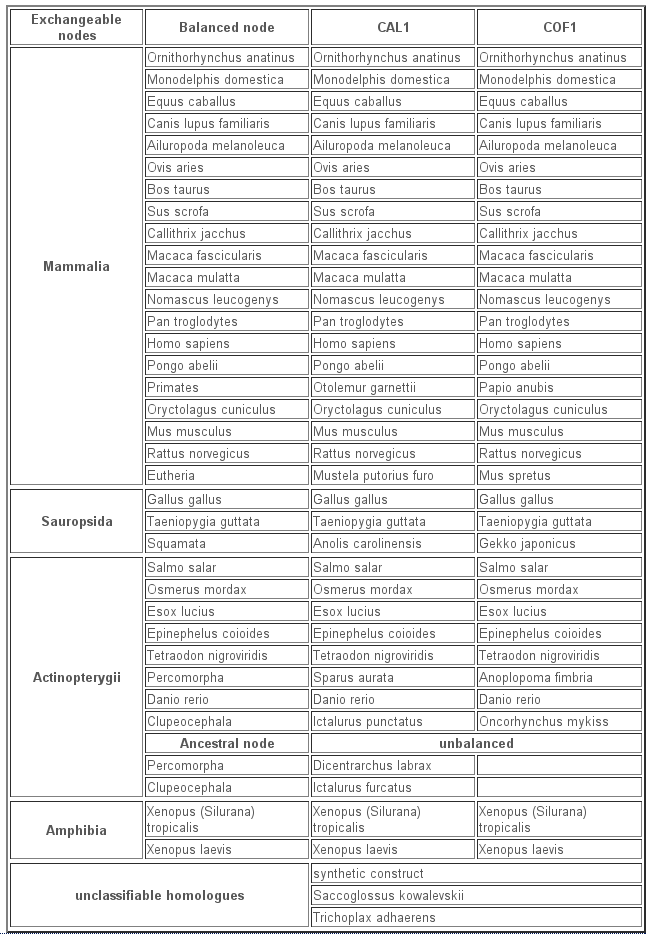
\includegraphics[width=5.4in]{figures/tablica.png}
\caption{Izlazna tablica s web stranice Orthobalancera}
\label{fig:tablica}
\end{figure}

Web aplikacija nakon izvođenja prikazuje tablicu balansiranih vrsta.  Stupci
tablice su imenovani po paralozima s ulaza. Retci su grupirani u zamjenske
čvorove. Svaki redak predstavlja jedan balansirani skup vrsta. U stupcu pod
pojedinim paralogom nalazi se ortologna vrsta, a lijevo od svih vrsta je zapisan
čvor na kojem su vrste tog retka balansirane. Primjer tablice se može vidjeti
na slici \ref{fig:tablica}.

Također, završna stranica sadrži poveznice za preuzimanje generiranih datoteka
tijekom izvođenja. Datoteke su opisane u nastavku.

Najvažnije izlazne datoteke su one koje sadrže poravnate sekvence ortologa iz
pojedine grupe ortologa. Za svaki ulazni paralog postoji datoteka imena
\emph{<ime-proteina>.afa}, gdje nastavak \emph{afa} ima konotaciju poravnata
FASTA \engl{aligned fasta}. Datoteke ovog tipa se mogu direktno preuzeti s
poveznice na završnoj stranici.

Nadalje, sa završne stranice se može preuzeti i \emph{zip} arhiva poravnatih
sekvenci, čije je ime oblika \emph{<PAR>\_OB\_fasta\_<D>\_<M>.zip}. \emph{<PAR>}
je ime prvog paraloga kojeg je korisnik unio, \emph{<D>} je dan, a \emph{<M>} je
mjesec kad je upit bio pokrenut. Budući da su zaglavlja izlaznih FASTA
sekvenci generirana tijekom rada Orthobalancera, ova \emph{zip} arhiva sadrži i
datoteke s dodatnim informacijama za svaku ortolognu sekvencu, imenovane
\emph{<ime-paraloga>\_orthologues.dict}. Svaka ortologna sekvenca će imati jednu
liniju u ovoj opisnoj datoteci sa sljedećim informacijama:

\begin{itemize}

    \item \emph{species name} ime vrste u kojoj se ova ortologna sekvenca
nalazi. Može se reći da ova sekvenca predstavlja navedenu vrstu jer između svih
pronađenih sekvenci koje pripadaju navedenoj vrsti, ova sekvenca ima najveći
rezultat sličnosti ulaznome paralogu.

    \item \emph{score} rezultat sličnosti ove sekvence prema ulaznome paralogu
dobiven iz izlaza alata BLAST.

    \item \emph{gid} jedan ili više identifikatora, odnosno FASTA ključeva ove
sekvence. Ispisani su ključevi koji identificiraju samo one proteine koji se
mogu naći u vrsti navedenoj u prvome stupcu.

\end{itemize}
Dodatno, ova \emph{zip} arhiva sadrži i datoteku \emph{similar\_species.txt}.
Ovdje je u tekstualnom obliku opisan sadržaj tablice na završnoj stranici. Na
početku su navedena imena paraloga. Nadalje, za svaki zamjenski čvor navedene su
grupe balansiranih vrsta popraćene s čvorom taksonomskog stabla na kojem su
vrste balansirane. Ukoliko se u nekoj balansiranoj grupi za neki paralog
pronašlo više ortologa, jedan se slučajnim odabirom prikazuje kao balansirani, a
ostali se prikazuju kao nebalansirani \engl{unbalanced} na kraju ispisa
pripadajućeg zamjenskog čvora. Na kraju datoteke je grupa vrsta koje su
pronađene za sve paraloge, ali se ne nalaze niti ispod jednog zamjenskog čvora.

\begin{sloppypar}

Na poslijetku, sa završne stranice se može preuzeti i \emph{zip} arhiva s
cjelokupnim sadržajem informacija prikupljenim tijekom pojedinog upita.
Imenovana je \emph{<PAR>\_OB\_<D>\_<M>.zip}, gdje je \emph{<PAR>}
ime prvog paraloga kojeg je korisnik unio, \emph{<D>} dan, a \emph{<M>}
mjesec pokretanja upita. Osim dosad spomenutih datoteka, ova arhiva sadrži još
sljedeće:

\end{sloppypar}

\begin{itemize}

    \item \emph{<ime-paraloga>.blast} izlaz alata BLAST za pojedini ulazni
paralog.

    \item \emph{<ime-paraloga>.fasta} sekvenca pojedinog paraloga u jednom
rektu bez zaglavlja

    \item \emph{<ime-paraloga>\_fastacmd.fasta} izlaz alata \emph{fastacmd}

    \item \emph{<ime-paraloga>\_orthologues.fasta} FASTA sekvence svih ortologa
pojedinog paraloga, neporavnate. Zaglavlje je generirano tijekom rada
Orthobalancera.

\end{itemize}
